\icode{E-MI-SI-L3-261108-001}
如图所示，倾斜直杆的左端固定在地面上，与水平面成\(\theta\)角，杆上穿有质量为\(m\)的小球\(a\)和轻质环\(b\)，两者通过一条细绳跨过定滑轮相连接。当\(a\)、\(b\)静止时，\(Oa\)段绳与杆的夹角也为\(\theta\)，不计一切摩擦，重力加速度为\(g\)。则下列说法正确的是\paren[]

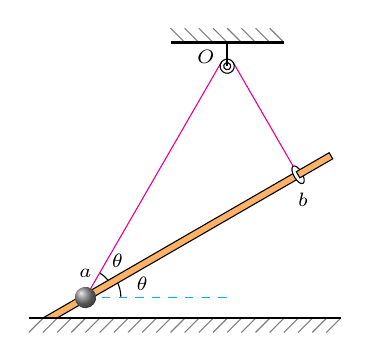
\begin{tikzpicture}[scale=.9,font=\scriptsize]
	\draw (60:.4) arc(60:30:.4);
	\draw (.5,0) arc(0:30:.5);
	\draw[dashed,cyan] (0,0)--(2,0);
	\begin{scope}[rotate=30]
		\coordinate (O) at({2*sqrt(3)-.1},{2-.1*sqrt(3)});
		\coordinate (E) at({2*sqrt(3)-.15},{2-.05*sqrt(3)});
		\coordinate (F) at({2*sqrt(3)},{2-.1*sqrt(3)});
		\draw[magenta] (0,0)--(E) (F)--({2*sqrt(3)},.1);
        \draw (O) circle(.1) (O) circle(.05);
		\draw[fill=orange!60] (0,-.05) rectangle({2*sqrt(3)},.05) (0,-.05)--(-.5,-.05)--++(150:.2)--(0,.05)--(0,-.05);
		\draw[fill=white] ({2*sqrt(3)},0) ellipse(.06 and .14);
		\draw[fill=orange!60] ({2*sqrt(3)},-.05) rectangle(4,.05);
		\shade[ball color=gray] (0,0) circle(.15);
		\node at({2*sqrt(3)},-.14)[below]{\(b\)};
	\end{scope}
	\foreach \x in {-.8,-.6,...,3.4}
		\draw[gray] (\x,{-.45-.025*sqrt(3)})--++(.2,.2);
	\foreach \x in {1.2,1.4,...,2.6}
		\draw[gray] (\x,3.8)--++(.2,-.2);
	\draw[thick] (-.8,{-.25-.025*sqrt(3)})--(3.6,{-.25-.025*sqrt(3)}) (O)--(O|-0,3.6) (1.2,3.6)--(2.8,3.6);
	\node at(.8,.2){\(\theta\)};
	\node at(.45,.52){\(\theta\)};
	\node at(0,.15)[above]{\(a\)};
	\node at(1.7,3.4){\(O\)};
\end{tikzpicture}
\begin{choices}
	\item\(b\)受杆的弹力方向垂直杆向上
	\item\(b\)受到杆的弹力大小为\(mg\tan\theta\)
	\item 绳对\(a\)的拉力大小为\(\frac{mg}{\tan\theta}\)
	\item 杆对\(a\)的支持力大小为\(mg\cos\theta\)
\end{choices}
\begin{answer}
	B\qquad 提示：
\end{answer}